\chapterfont{\color{DarkOrange}}  % sets colour of chapter
\sectionfont{\color{DarkOrange}}  % sets colour of sections
\subsectionfont{\color{DarkOrange}}  % sets colour of subsections

\renewcommand\pcolor{DarkOrange}
\renewcommand{\headrule}{\hbox to\headwidth{%
		\color{DarkOrange}\leaders\hrule height \headrulewidth\hfill}} % color of title
\fancyfoot[LE,RO]{\thepage}

{ \Large \leftwatermark{
		\put(-67,-66.5){ 1 }
		\put(-67,-91.5){ 2 }
		\put(-67,-116.5){ 3 }
		\put(-67,-141.5){ 4 }
		\put(-76.5,-176){
\includegraphics[scale=0.8]{img/thumbindex/thumbindex_DarkOrange.eps}} 
		\put(-67,-166.5){{\color{white} 5 }}
		\put(-67,-191.5){ 6 }
	} \rightwatermark{
		\put(350.5,-66.5){ 1 }
		\put(350.5,-91.5){ 2 }
		\put(350.5,-116.5){ 3 }
		\put(350.5,-141.5){ 4 }
		\put(350.5,-176){
\includegraphics[scale=0.8]{img/thumbindex/thumbindex_DarkOrange.eps}} 
		\put(350.5,-166.5){ {\color{white} 5 } }
		\put(350.5,-191.5){ 6 }
}}

\chapter[Cis- and trans-eQTL analysis in brain cortex reveals distinct regulatory effects of disease-associated genetic variants]{Cis- and trans-eQTL analysis in brain cortex reveals distinct regulatory effects of disease-associated genetic variants}
\chaptermark{}

\label{chap:chapter5-brain}

\noindent
\\
\\

Niek de Klein\textsuperscript{1,4,5,6}, Ellen A. Tsai\textsuperscript{2,6}, Martijn Vochteloo\textsuperscript{1,3,7}, Denis Baird\textsuperscript{2,7}, Yunfeng Huang\textsuperscript{2}, Chia-Yen Chen\textsuperscript{2}, Sipko van Dam\textsuperscript{1}, Omar El Garwany\textsuperscript{1,5}, Maria Zavodszky\textsuperscript{2}, Heiko Runz\textsuperscript{2,8}, Lude Franke\textsuperscript{1,4,8}, Harm-Jan Westra\textsuperscript{1,4,8}






\noindent
1. Department of Genetics, University Medical Center Groningen, University of Groningen, Hanzeplein 1, Groningen, The Netherlands \\
2. Translational Biology, Research \& Development, Biogen Inc., 225 Broadway, Cambridge, MA, USA \\
3. Institute for Life Science \& Technology, Hanze University of Applied Sciences, Zernikeplein 11, 9747 AS Groningen, The Netherlands \\
4. Oncode Investigator \\
5. Wellcome Sanger Institute, Wellcome Genome Campus, Hinxton, UK \\
6. These authors contributed equally \\
7. These authors contributed equally \\
8. These authors jointly supervised the work 
\\
\\

\newpage

\section*{Abstract}
Gaining insight into the downstream consequences of non-coding variants is an essential step towards the identification of therapeutic targets from genome-wide association study (GWAS) findings.  Here we have harmonized and integrated 8,727 RNA-seq samples with accompanying genotype data from multiple brain-regions from 14 datasets. This sample size enabled us to perform both cis- and trans-expression quantitative locus (eQTL) mapping. Upon comparing the brain cortex cis-eQTLs (for 12,307 unique genes at FDR $<$ 0.05) with a large blood cis-eQTL analysis (n=31,684 samples), we observed that brain eQTLs are more tissue specific than previously assumed. 

We inferred the brain cell type for 1,515 cis-eQTLs by using cell type proportion information. We conducted Mendelian Randomization on 23 neurological traits using the cis-eQTLs and found 159 significant findings that also passed colocalization. Of the 20 Multiple Sclerosis (MS) MR findings, three genes did not have a significant eQTL in blood tissue, underscoring the importance of building and using tissue-specific resources. Furthermore, two MS findings had cell-type specific signals, a neuron-specific cis-eQTL for CYP24A1 and a macrophage specific cis-eQTL for CLECL1.  

To further interpret GWAS hits, we performed trans-eQTL analysis. We identified 2,589 trans-eQTLs (at FDR $<$ 0.05) for 373 unique SNPs, affecting 1,263 unique genes, and 21 replicated significantly using single-nucleus RNA-seq data from excitatory neurons.  

We also generated a brain-specific gene-coregulation network that we used to predict which genes have brain-specific functions, and to perform a novel network analysis of MS, Alzheimer’s disease, Parkinson’s disease and amyotrophic lateral sclerosis GWAS data. This resulted in the identification of distinct sets of genes that show significantly enriched co-regulation with genes inside the associated GWAS loci, and which might reflect drivers of these diseases. 

All eQTL summary statistics and the brain specific co-regulation network are publicly available at \url{www.metabrain.nl}. 

\section{Introduction}
The world health organization estimates that 329 million individuals were affected by psychiatric diseases depression, bipolar disorder, and schizophrenia in 2017\cite{jamesGlobalRegionalNational2018}. Additionally, with increasing life expectancy, the number of patients with neurodegenerative diseases, such as Alzheimer’s disease or Parkinson’s disease is steadily increasing: currently there are 50 million people living with dementia worldwide, which is expected to rise to 152 million by 2050\cite{WorldAlzheimerReport2018}. While the genetic aspects for these psychiatric and neurodegenerative diseases are currently being uncovered by genome-wide association studies (GWAS), much of how the identified genetic variants affect the brain is still unknown. 

To identify potential mechanisms, associations with gene expression levels, or expression quantitative trait loci (eQTL) have shown great potential. eQTLs can be divided in direct effects of local genetic variants (\emph{cis}-eQTLs) and indirect effects of distal variants (\emph{trans}-eQTLs). Considering that the results of recent GWAS suggest that complex diseases and traits may be more polygenic than initially thought, \emph{cis}-eQTLs, and \emph{trans}-eQTLs can aid interpretation in several ways: \emph{cis}-eQTLs by identifying direct links between genes and phenotypes through approaches such as colocalization analysis and Mendelian Randomization (MR), and \emph{trans}-eQTLs by exposing sets of core genes and pathways on which the effects of disease variants converge.  

eQTLs are complex associations that can be dependent on tissue, cell-type, stimulation, and other phenotypes (gender, age, interferon-status, etc). For proper interpretation of GWAS associations, it is therefore essential to perform eQTL analyses in disease relevant tissues. To interpret neurodegenerative and psychiatric disorders, several large brain-derived eQTL studies have been published recently, including meta-analyses by the PsychENCODE\cite{wangComprehensiveFunctionalGenomic2018}, and AMP-AD\cite{rajIntegrativeTranscriptomeAnalyses2018} consortia, covering 1,866 and 1,433 individuals, respectively. However, interpretative approaches such as colocalization and MR need errors of effect size estimates to be small, requiring even larger eQTL sample sizes. 

To maximize the potential of such interpretative analyses in brain, we therefore combined and rigorously harmonized existing brain RNA-seq and genotype data from 15 different cohorts: we included publicly available samples from the European Nucleotide Archive (ENA) and all major brain eQTL studies. Using this resource, we created a gene coregulation network consisting of 8,614 RNA-seq samples covering different brain regions and performed cis- and trans-eQTL analysis in up to 2,970 individuals from European descent, with replication in up to 420 individuals of African descent. For cortex, we identified 11,803 significant primary cis-eQTL genes, 41\% of which had a significant secondary association in a conditional analysis. Furthermore, we identified 1,263 trans-eQTL genes in cortex. We then applied genome-by-environment (GxE) interaction analysis, and prioritized oligodendrocytes and neurons as the main driver cell types for cis-eQTL effects (\textbf{Figure 1}): we identified 1,515 and 126 cell count interaction eQTLs in cortex and cerebellum, respectively. Finally, we used our results to prioritize disease associated genes by applying Mendelian Randomization and colocalization using GWAS results for various neurological phenotypes.  

By rigorous harmonization and by combining the statistical power across these datasets, our resource provides the next step in the application of gene expression levels to understand neurodegenerative and psychiatric disease. To facilitate future studies, we have made all summary statistics and the generated co-expression network available through https://www.metabrain.nl/. 

\begin{figure}[h!]
	\includegraphics[width=\textwidth]{chapters/chapter5-brain-eqtls/img/2020-10-07-fig1-abstract_figure_v7.pdf}
	\caption{\textbf{Overview of the study.} We downloaded publicly available RNA-seq and genotype data from 15 different datasets consisting of 6,518 individuals, with measurements from 7 main brain regions.  After QC, normalization and covariate correction, the first two PC’s on the gene quantification data shows that the samples are clustering on brain region. Subsequently, we performed cis-, trans, and interaction-eQTL analysis, build a Subsequently, we performed \emph{cis}-, \emph{trans}, and interaction-eQTL analysis, build a brain-specific gene coregulation network and performed mendelian randomization.}
\end{figure}


\section{Results}
\subsection{Leveraging public RNA-seq and genotype data to create large, harmonized brain eQTL and gene co-regulation datasets}
In recent years, many brain-derived eQTL datasets have been published. Here, we opted to combine these datasets in order to provide an increase in statistical power to detect eQTLs, and to create a brain specific gene coregulation network. We coin our resource ‘MetaBrain'. To create this resource, we first retrieved brain-derived RNA-seq and genotype datasets from multiple previously published and private datasets (\textbf{Supplementary Table 1}; \textbf{Figure 2A-C}), including 7,604 samples from the AMP-AD consortium\cite{hodesAcceleratingMedicinesPartnership2016} (AMP-AD MAYO\cite{hodesAcceleratingMedicinesPartnership2016}, ROSMAP\cite{hodesAcceleratingMedicinesPartnership2016} and MSBB\cite{hodesAcceleratingMedicinesPartnership2016}), Braineac\cite{ramasamyGeneticVariabilityRegulation2014}, the PsychENCODE consortium\cite{consortium*RevealingBrainMolecular2018} (Bipseq\cite{wangComprehensiveFunctionalGenomic2018}, BrainGVEX\cite{wangComprehensiveFunctionalGenomic2018}, CMC\cite{fromerGeneExpressionElucidates2016}, GVEX, and UCLA\_ASD\cite{wangComprehensiveFunctionalGenomic2018}), BrainSeq\cite{brainseq2015}, NABEC\cite{gibbsAbundantQuantitativeTrait2010}, TargetALS\cite{prudencioDistinctBrainTranscriptome2015}, and GTEx\cite{donovanCellularDeconvolutionGTEx2020} To further expand this dataset, we carefully selected 1,759 brain RNA-seq samples from the European Nucleotide Archive (ENA)\cite{leinonenEuropeanNucleotideArchive2011}. For this purpose, we used the SkyMap\cite{tsuiExtractingAllelicRead2018} database for initial tissue annotation and PCA to identify additional, previously unannotated, brain samples (\textbf{Supplementary Note}). This resulted in a combined dataset consisting of 9,363 RNA-seq samples. Next, we uniformly realigned the samples and performed rigorous quality control using PCA and technical covariates, resulting in a final dataset consisting of up to 8,727 samples.  

We grouped the RNA-seq samples into 7 major tissue groups (amygdala, basal ganglia, cerebellum, cortex, hippocampus, hypothalamus and spinal cord; \textbf{Supplementary Table 1}). PCA on the final dataset showed clear clustering of major brain tissue groups, which loosely resembled the relative spatial distances of each tissue type based on brain physiology (\textbf{Figure 2E}) rather than differences between datasets (\textbf{Figure 2D}), indicating we properly corrected for dataset-specific technical variation, which we then used to define a set of 86 amygdala, 574 basal ganglia, 723 cerebellum, 6,601 cortex, 206 hippocampus, 252 hypothalamus and 285 spinal cord samples (\textbf{Supplementary Table 1}, \textbf{Figure 2A}). 

Next, we evaluated the available genotype datasets. The collected datasets contained genotypes generated using different platforms, including genotypes called from whole genome sequencing (WGS; AMP-AD\cite{hodesAcceleratingMedicinesPartnership2016}, TargetALS\cite{prudencioDistinctBrainTranscriptome2015}, GTEx\cite{donovanCellularDeconvolutionGTEx2020}), genotyping arrays (NABEC\cite{DbGaPStudy}, Braineac\cite{ramasamyGeneticVariabilityRegulation2014}), and haplotype reference consortium (HRC)\cite{mccarthyReferencePanel642016} imputed genotypes (PsychENCODE datasets). Sample genotype was not available for samples retrieved from ENA, so we performed genotype calling using the RNA-seq reads using the GATK\cite{mckennaGenomeAnalysisToolkit2010} pipeline (Supplementary Note). We identified individuals from many different ethnicities using the genotype data (\textbf{Supplementary Figure 1}): 5,138 samples had European (EUR) ancestry, 805 samples had African (AFR) ancestry, and 573 samples were assigned to other ethnicities (\textbf{Supplementary Table 1}, \textbf{Figure 2B}). 

We were able to determine 7,644 links between RNA-seq samples and genotyped individuals, reflecting 3,525 unique EUR individuals, 624 unique AFR individuals, and 510 unique individuals assigned to other ethnicities. For the purpose of eQTL analysis, we focused on datasets having at least 30 uniquely linked individuals for a tissue and ethnicity group. We were able to create 7 eQTL discovery datasets: Basal ganglia-EUR (n=208), Cerebellum-EUR (n=492), Cortex-EUR (n=2,970), Cortex-AFR (n=420), Hippocampus-EUR (n=168) and Spinal cord-EUR (n=108; \textbf{Supplementary Table 1}, \textbf{Figure 2C}). 

\begin{figure}[H]
	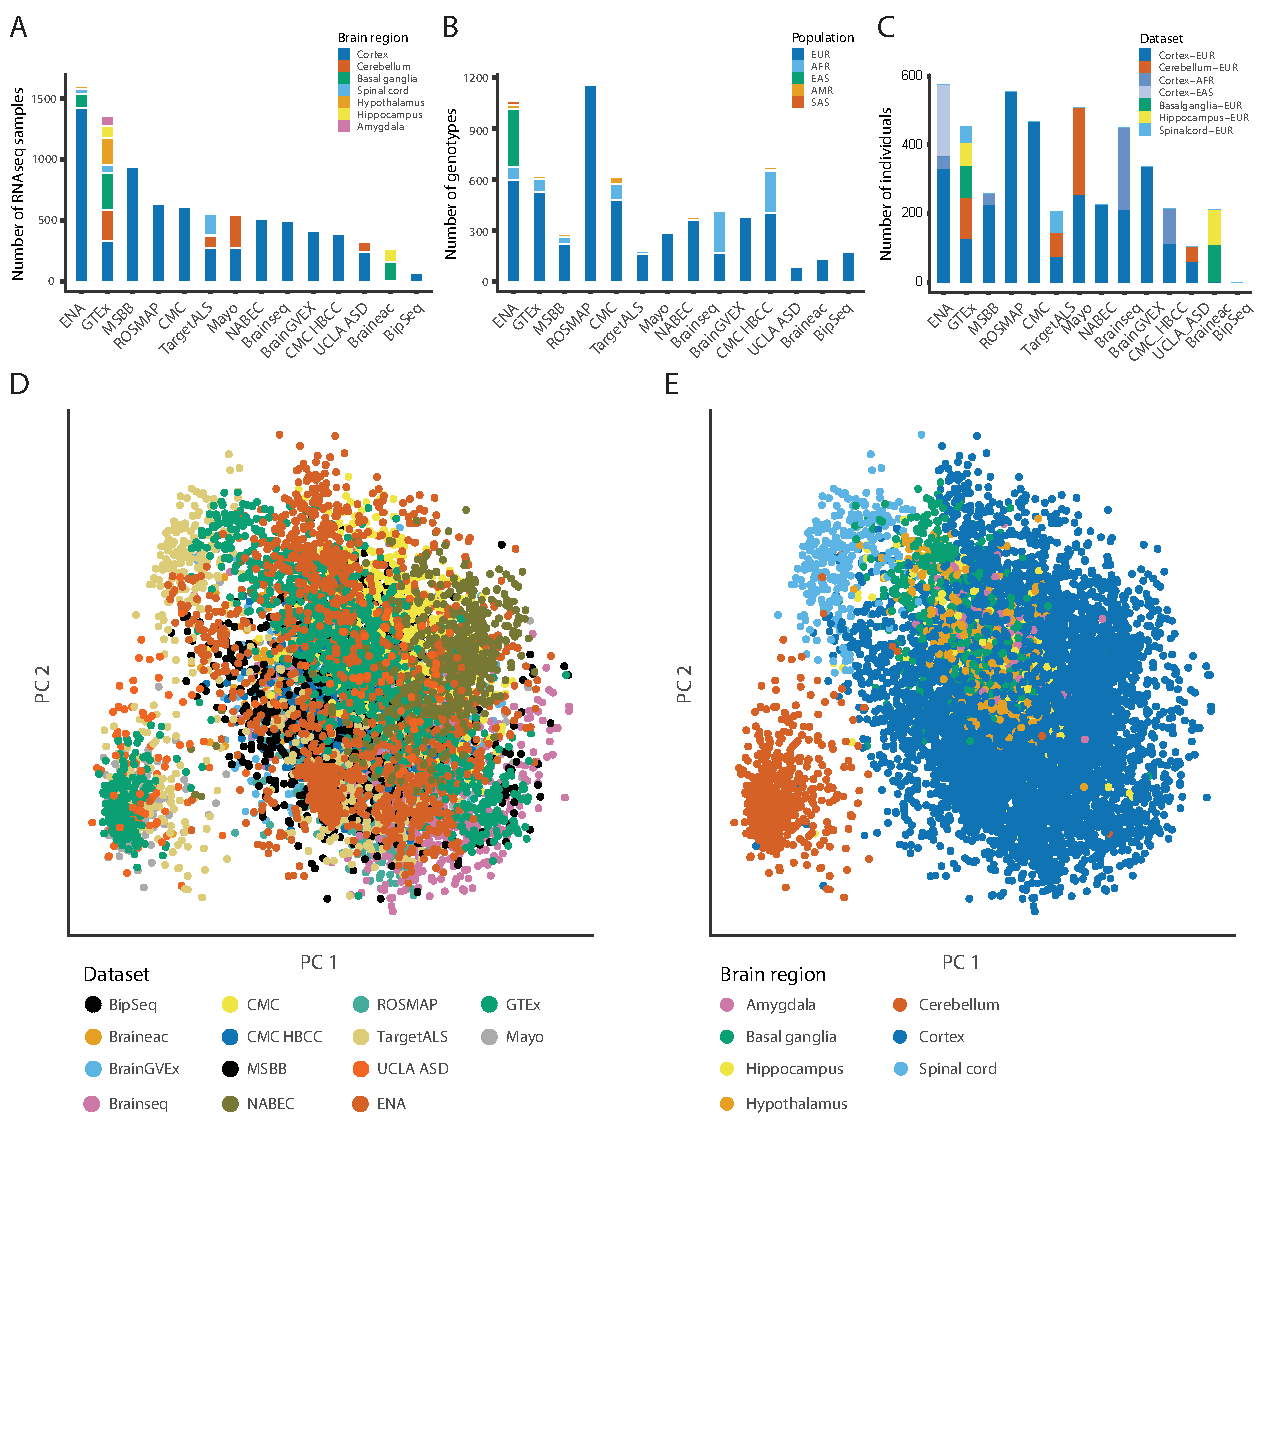
\includegraphics[width=\textwidth]{chapters/chapter5-brain-eqtls/img/2020-07-09-fig2-datasetoverview-v5.pdf}
	\caption{\textbf{Overview of the dataset.} (A) The number of samples per included cohort, with each color representing one of the 7 major brain regions. (B) The number of genotypes per cohort, with each color representing a population. (C) The number of individuals per cohort, with each color representing an eQTL dataset. The number of individuals is different from the intersection between the number of RNA-seq samples and number of genotypes, because not all samples with genotypes have RNA-seq samples and vice-versa, and some indviduals with genotypes have multiple RNA-seq measurements. (D) PC1 and PC2 of the normalized expression data after covariate correction colored by cohort shows that cohorts are not clustering together, meaning that most cohort specific batch effects have been removed. (E) The same PCA as D, but colored by brain region shows that the clustering is mainly on brain region, and that is difficult to distinguish between cortex, hypothalamus, basal ganglia, and amygdala.}
\end{figure}

\subsection{Co-regulation network }
For many genes that are identified to be involved with neurological or psychiatric disorders through eQTL or other studies there is no known function available yet. The function of these genes of interests can be inferred through functional enrichment tools such as Enrichr\cite{chenEnrichrInteractiveCollaborative2013,EnrichrComprehensiveGene}, ToppGene\cite{chenToppGeneSuiteGene2009}, or GeneNetwork\cite{deelenImprovingDiagnosticYield2019}. However, these functional enrichment tools usually include samples from multiple tissues, of which only a small part is from samples in the brain. To improve the specificity of genes related to disorders of the brain, we created a co-regulation network with 8,544 samples that passed the quality control for the eQTL analysis. For 6 types of gene set databases (KEGG\cite{kanehisaKEGGKyotoEncyclopedia2000}, REACTOME\cite{jassalReactomePathwayKnowledgebase2020}, HPO\cite{kohlerExpansionHumanPhenotype2019}, GO Molecular Function\cite{kohlerExpansionHumanPhenotype2019}, GO Biological ProcesskohlerExpansionHumanPhenotype2019, and GO Cellular ComponentkohlerExpansionHumanPhenotype2019) coregulation and gene set predictions were performed using the GeneNetwork method\cite{deelenImprovingDiagnosticYield2019}. It is possible to search for a gene, or a set of genes on http://www.metabrain.nl/. 

\subsection{cis-eQTL discovery and replication }
Within each discovery dataset, we performed a sample-size weighted \emph{cis}-eQTL meta-analysis, assessing variants with minor allele frequency (MAF) $>$ 0.01 and Hardy-Weinberg $p > 1 \times 10^{4})$ within 1 megabase (Mb) of the transcription start site (TSS) of a protein-coding gene. We considered eQTLs with an FDR $<$ 0.05, determined using permutations, as significant. We identified 1,317 (Basal ganglia-EUR), 6,865 (Cerebellum-EUR), 5,440 (Cortex-AFR), 11,803 (Cortex-EUR), 990 (Hippocampus-EUR), and 811 (Spinal cord-EUR) cis-eQTLs genes (\textbf{Figure 3A}; \textbf{Table 1}). When comparing eQTL effect directions between Cortex datasets, we observed high rates of concordance and correlation of association Z-scores (Spearman r $>$ 0.59; allelic concordance $>$ 72\%; \textbf{Supplementary Figure 2}), indicating robustness of the identified effects across datasets.  

\subsection{41\% of the cortex eQTL genes are regulated by multiple independent variants}
\emph{Cis}-eQTL loci are known to often harbor multiple independent associations\cite{aguetGeneticEffectsGene2017,zhernakovaIdentificationContextdependentExpression2017,vosaUnravelingPolygenicArchitecture2018}. To identify additional independent \emph{cis}-eQTLs signals, we performed an iterative conditional analysis (See Methods). Using this approach, we identified 4,791 significant secondary (41\% of \emph{cis}-eQTL genes identified in this dataset), 1,658 tertiary and 598 quaternary \emph{cis}-eQTLs in the Cortex-EUR dataset. Similarly, we identified secondary associations for the other discovery datasets albeit to a lesser extent due to the limited sample sizes of these datasets (\textbf{Figure 3A}, \textbf{Table 1}).  

In blood, it has been shown that over 90\% of highly expressed genes are \emph{cis}-eQTL genes, and genes without a \emph{cis}-eQTL have low tolerance for loss of function mutations\cite{vosaUnravelingPolygenicArchitecture2018}. In contrast, in our cortex data, we observed that many highly expressed genes are not eQTL genes: the median expression level of primary eQTL genes (median $log_2$(TMM) expression=2.511) was slightly, but significantly, higher than that of genes without a \emph{cis}-eQTL (median expression=2.505, Wilcoxon p-value: 9.96x10-12). Comparing genes having only a primary eQTL association (median expression=2.596) with those having a secondary eQTL, we observed that genes with a secondary eQTL generally had a lower median expression level (median $log_2$(TMM) expression=2.388; Wilcoxon p-value = $1.3 \times 10^{-25}$). Genes with additional independent eQTL associations showed a further decrease in median expression level (\textbf{Figure 3B}, left). Furthermore, we observed that even though primary eQTL genes had higher mean expression than non-primary genes, their standard deviation was lower(\textbf{Supplementary Figure 3A}). 

The distance between the eQTL variant and the transcription start site (TSS) shifts further away with additional independent eQTL associations: primary eQTLs had a median distance of 31kb, secondary eQTLs a median distance of 42kb, tertiary eQTLs a median distance of 53kb, and quaternary eQTLs a median distance of 76kb (\textbf{Figure 3B}, middle). Although we did observe a shift in distance between eQTL variant and TSS, the shift is smaller than that of previously published results in cortex\cite{dobbynLandscapeConditionalEQTL2018}.  

In blood, genes with low tolerance for loss of function mutations, as indicated by the pLI score, are less likely to be eQTL genes\cite{vosaUnravelingPolygenicArchitecture2018}. In cortex, we observed a similar pattern, with genes having a primary eQTL having lower pLI scores than those without ($\chi^2$ p=6.35x10-147). This effect was smaller but still significant for secondary ($\chi^2$ p= 4.4x10-43) and tertiary eQTLs ($\chi^2$ $p = 3.7 \times 10^{-06}$), but not for quaternary eQTLs ($\chi^2$ p$>$0.05, \textbf{Figure 3B}, right). 

Functional enrichment showed little difference between the types of eQTLs, with both primary and non-primary genes being enriched for autosomal recessive disorders (HPO). However, primary genes did have strong enrichments for protein binding (GO molecular function), intracellular and cytoplasm (GO cellular component) (\textbf{Supplementary Figure 3C}), while non-primary genes were enriched for catalytic activity (GO molecular function). Finally, primary eQTL genes had many more TRANSFAC\cite{wingenderTRANSFACDatabaseTranscription1996} transcription factor motifs enriched. See \textbf{Supplementary Table 6} for a full list of significant enrichments.    

\begin{figure}[H]
	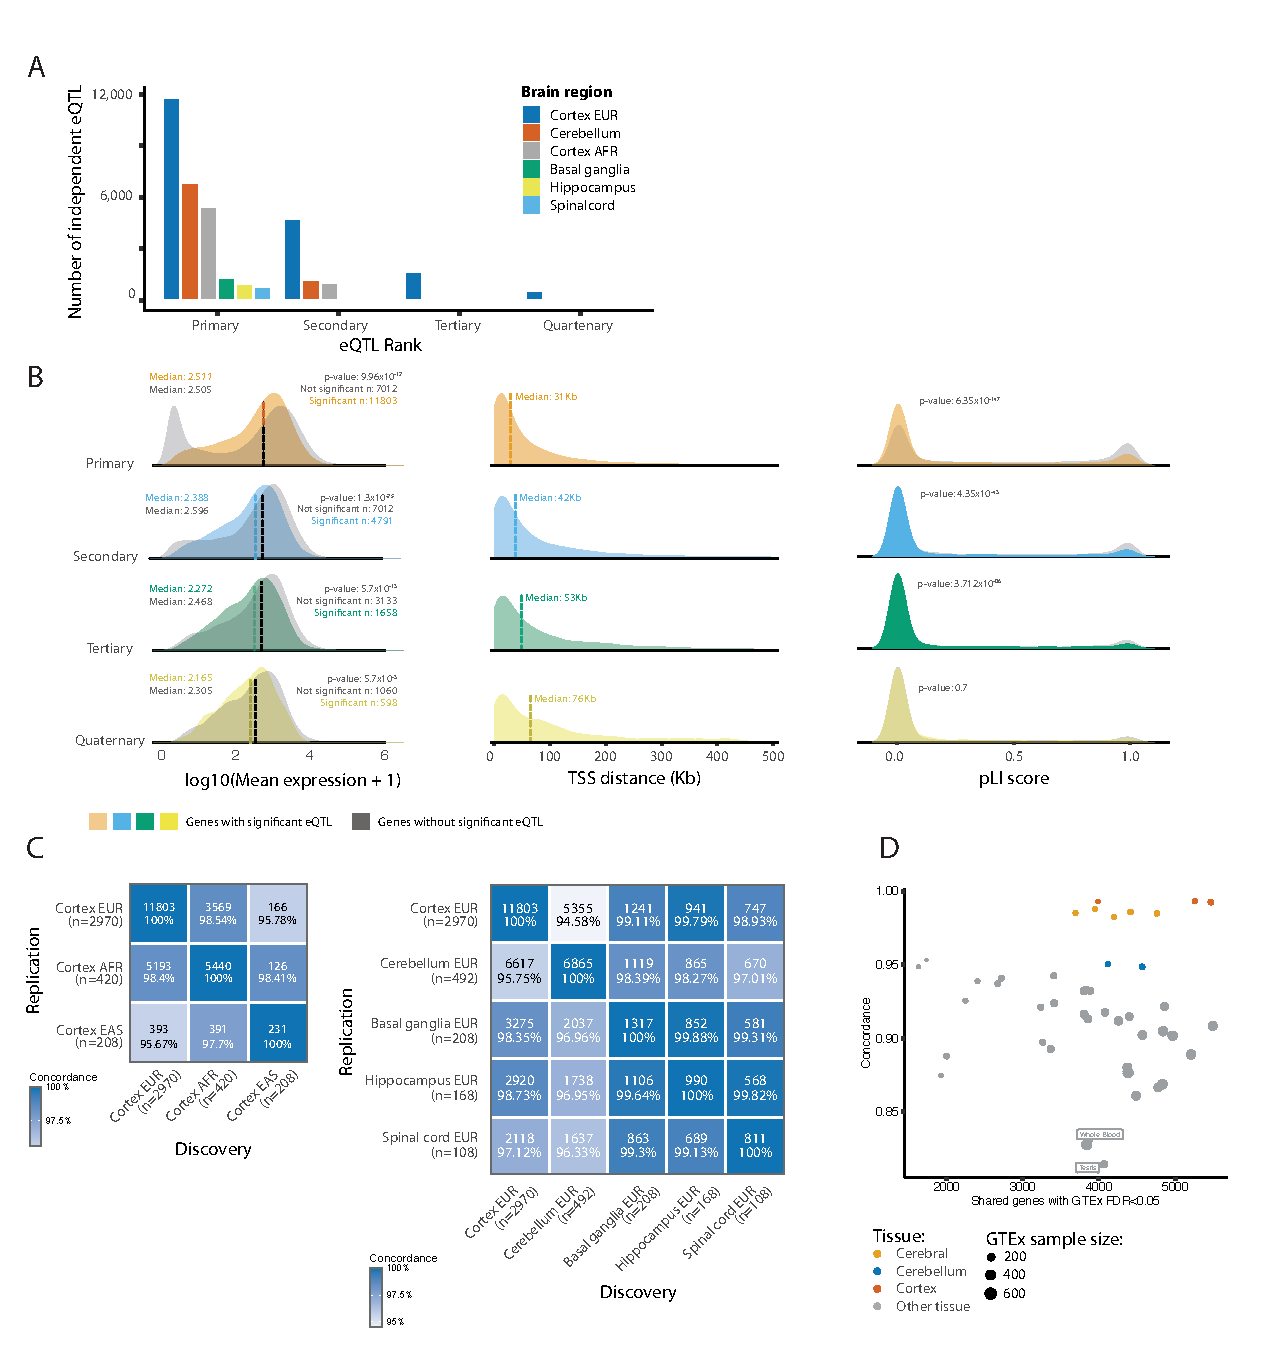
\includegraphics[width=\textwidth]{chapters/chapter5-brain-eqtls/img/2020-12-02-fig3-ciseqtls-v12.pdf}
	\caption{\textbf{Figure 3. Conditional cis-eQTLs.} (A) The number of conditional cis-eQTLs per eQTL dataset. (B) Replication of primary cis-eQTLs between; (left) the cortex eQTLs of different ethnicities (left) and; (right) the different brain regions for the European datasets. The n under the dataset name is the number of samples in that dataset. The boxes show the number the number of eQTLs that are significant in both the discovery and the replication set, and the percentage of those that shows the same direction of effect. (C) The replication between primary cis-eQTLs of Cortex-EUR (discovery) with all the GTEx tissues (replication). Each dot is a different GTEx tissue, the x-axis is the number of eQTLs that is signifcant in both discovery and replication, and the y-axis is the percentage that shows the same direction of effect. (D) Comparison of characteristics between primary and non-primary eQTLs. (left) The difference in mean expression; (middle) the difference in distance between the most significant SNP-gene combination; (right) the difference in pLI score.}
\end{figure}

\subsection{Cis-eQTLs have high allelic concordance between ethnicities and brain regions }
Tissue specific\cite{aguetGeneticEffectsGene2017}, brain region specific\cite{siebertsLargeEQTLMetaanalysis2020}, and to a lesser extent, population specific\cite{shangGeneticArchitectureGene2020} eQTLs have been observed in previous reports. Our dataset allowed us to evaluate the influence of these factors on eQTL concordance, by comparing the discovered eQTLs between different brain tissues and ethnicities. For cortex, we performed discovery in EUR and AFR datasets, and had access to a smaller East-Asian (EAS) dataset (208 samples) that was excluded from discovery since these individuals were limited to the ENA dataset. Discovery in the EUR population and replication in AFR and EAS populations showed high concordance in the AFR population (5,193 eQTLs significant in both datasets, 98.4\% with same allelic direction), and the EAS population (391 eQTLs significant in both datasets, 95.67\% with same allelic direction). Discovery in the AFR population and replication in the EAS population showed a high concordance in direction of effect as well (391 eQTLs significant in both datasets, 97.7\% with same allelic direction), although the difference was not significant (Fisher exact p = 0.34). Discovery in the EAS population and replication in EUR and AFR populations showed that concordance in direction of effect was high for cis-eQTLs that were significant in both replication datasets ($>$95\%; \textbf{Figure 3C}). These results indicate that the sample size per cohort strongly determines how many \emph{cis}-eQTLs can be found and determines what fraction replicates significantly in another population. Additionally, these results indicate that eQTLs from the same tissue that are significant across populations generally share the same allelic direction. 

Similarly, within the EUR population cohorts we studied how well cis-eQTLs identified in one brain region can replicate in other brain regions. We observed high concordance of allelic directionality across brain tissue types. Despite having the second largest sample size, cerebellum had the lowest concordance with other brain regions (94.58\%, 96.96\%, 96.95\%, 96.33\% for Cortex-EUR, Basal ganglia, Hippocampus, and Spinal cord, respectively, \textbf{Figure 3C}). This might suggest a difference in genetic regulation between cerebellum and other tissues of the brain.  

Although the concordance of the shared eQTL effects was high between brain regions, a substantial number of eQTL genes were only found in one region. For example, in Cortex-EUR, we identified 5,514 unique eQTL genes (\textbf{Supplementary Figure 4A}). This large number of unique Cortex-EUR eQTLs is likely due to the difference in sample size between brain regions, and we expect to find more shared effects when sample sizes would increase for the other tissues. We also found 846 unique Cerebellum eQTL genes (\textbf{Supplementary Figure 4A}), which we reasoned were less likely due to sample size differences, as Cortex-EUR has a 7-fold higher sample size. For most of these genes (690/846), the expression in Cortex-EUR was lower than in Cerebellum (\textbf{Supplementary Figure 4B}). Although lower expression of a gene in cortex can explain why no eQTL is found, many genes were still highly expressed in cortex and would therefore be expected to show an eQTL effect.  

Another possible reason for missing eQTLs is that these genes are regulated by transcription factors only found in cerebellum. To test this, identified transcription factors enriched for regulating the genes highly expressed in cortex but not showing a cortex eQTL. We divided the eQTLs in low and high expressed genes. Since the cortex expression of these 846 genes follows a bimodal distribution, we selected high expressed genes as those on the right of the minimum ($log_2$(TMM+1) $<$ 4) of this bimodal distribution (\textbf{Supplementary Figure 4C}). These 681 highly expressed genes were enriched for many transcription factor binding sites. Nine of these transcription factors (EOMES, TFAP2B, IRX1, IRX5, HES7, ETV2, ELF3, and RUNX3) are highly expressed in cerebellum ($log_2$(TMM+1) $>$ 4) and lower ($log_2$(TMM+1) $<$ 4) in cortex. This difference in transcription factor expression might explain why these eQTLs are found in the Cerebellum dataset but not in the larger sample size Cortex dataset. 

Finally, we tested if the functions of these genes were enriched for <FILL IN> (\textbf{Supplementary Figure X}, \textbf{Supplementary Table X}), which is expected for a set of genes that is expressed in the brain. We also observed many enrichments for transcription factor binding sites. Four of these transcription factors (EOMES, TFAP2B, IRX1 and IRX5) are highly expressed in Cerebellum ($log_2$(TMM+1) $>$ 5) and much lower ($log_2$(TMM+1) $<$ 2) in Cortex. This difference in transcription factor expression might explain why these eQTLs are found in the Cerebellum dataset but not in the larger sample size Cortex dataset. 

To evaluate whether the high rate of sharing between tissues was a persistent observation, we repeated the Cortex-EUR discovery, while omitting GTEx samples, and subsequently attempted replication of the discovered cis-eQTLs in the different GTEx tissues\cite{consortiumGTExConsortiumAtlas2020}. Cerebral and cortex regions of the brain had highest directional concordance with Cortex-EUR eQTLs ($>$99\%), while concordance in cerebellum was more comparable to other, non-brain, tissues (\textbf{Figure 3D}, \textbf{Supplementary Figure 5}; \textbf{Supplementary Table 3}). As expected, the overall allelic concordance was highest in GTEx brain samples ($>$90\%), and the lowest concordances observed was in testis (84\%) and whole blood (85\%). We also quantified the number of concordant eQTLs with eQTLgen, a large blood-based dataset (n=31,684). Replicating eQTLs identified in our study in eQTLgen resulted in an allelic concordance of only 76\% for Cortex-EUR: thus 24\% of the shared eQTLs between blood and brain show opposite allelic effects. Since the procedures for eQTL mapping were identical, we conclude that when eQTL cohort sample-sizes become large it becomes apparent that there is strong tissue-specific regulation, which can explain these opposite allelic effects\cite{fuUnravelingRegulatoryMechanisms2012} (\textbf{Supplementary Figure 6}). 

Together with the replication results in GTEx, this suggests that many Cortex-EUR eQTLs may be shared with other tissues, but also that there is a considerable fraction of eQTLs that may be under different genetic control. We therefore next attempted to identify Cortex-EUR specific eQTLs by conditioning on previously identified eQTLs, including all independent associations per gene, where available. When we regressed out 45,748 blood-based eQTLs from BIOS\cite{zhernakovaIdentificationContextdependentExpression2017} (for which additional independent eQTLs signals were available) and eQTLgen, we observed that <CHANGE xyz CHANGE> genes remained with a significant (FDR$<$0.05) cis-eQTL in cortex. To further account for eQTLs shared by multiple tissues, we next conditioned on an additional 400,633 eQTLs from all GTEx tissues except brain, after which 1,594 genes remained significant in Cortex-EUR.

\subsection{8\% of Cortex cis-eQTLs are mediated by cell type proportion differences}
	
Apart from population and tissue dependence, eQTLs are also known to be cell type dependent. We\cite{raulaguirregamboaDeconvolutionBulkBlood2020}, and others\cite{donovanCellularDeconvolutionGTEx2020,glastonburyCellTypeHeterogeneityAdipose2019}, have shown previously that cell type dependent eQTLs can be detected in bulk RNA-seq datasets by first performing cell type deconvolution to estimate cell type proportions, and calculating eQTL-cell type proportion interaction effects.  

We predicted the five major cell types of the brain (neurons, oligodendrocytes, macrophages, endothelial cells, and astrocytes) using single cell RNA-seq profiles from each respective cell type. In cortex, we predicted neurons to be the most abundant (median cell count proportion of 32.8\%), followed by endothelial cells (24.9\%), macrophages (17.8\%), oligodendrocytes (12.4\%), astrocytes (12.1\%; \textbf{Supplementary Figure 7}). Predicted cell proportions were negatively correlated between neurons and the other cell types (Spearman r $<$ -0.14), and between endothelial cells and macrophages (Spearman r $<$ -0.32) in both Cortex and Cerebellum (\textbf{Figure 4A}). As a validation, we compared cell type proportions predicted in ROSMAP with immunohistochemistry (IHC) counts available for 42 samples of this dataset\cite{patrickDeconvolvingContributionsCelltype2020} (\textbf{Figure 4B}). We observed positive correlations for all cell types (Spearman r $>$ 0.1), and the scale of predicted proportions was comparable with those observed in IHC data. One exception was neurons, for which the IHC data showed higher average counts than our predictions, perhaps caused by the fragile nature of these cell types in post-mortem samples. In cerebellum, we also predicted neurons to be the most common cell type (median cell count proportion of 32.8\%), followed by endothelial cells (27.5\%), macrophages (14.7\%), oligodendrocytes (13.3\%), astrocytes (11.5\%; \textbf{Supplementary Figure 7}). We do note however, that there is no clear consensus on the expected percentage for each cell type, which makes it difficult to validate the predictions\cite{herculano-houzelHumanBrainNumbers2009,vonbartheldSearchTrueNumbers2016}. 

After predicting cell type proportions, we applied them to identify cell type interaction eQTLs (ieQTLs) in Cortex-EUR and Cerebellum-EUR using DeconQTL\cite{raulaguirregamboaDeconvolutionBulkBlood2020}. We tested a total of 18,850 and 8,347 cis-eQTLs in Cortex-EUR and Cerebellum samples, respectively, including primary, secondary, tertiary and quaternary independent associations. For Cortex-EUR, we identified 1,515 significant ieQTLs (8\%) in at least one cell type (Benjamini Hochberg; BH FDR $<$ 0.05). We observed the largest number of ieQTLs for neurons (632), likely because this is the most prevalent cell type. The majority (90.2\%) of the ieQTLs were uniquely mapped to one cell type (\textbf{Figure 4C}).  For Cerebellum, we identified 126 significant ieQTLs (1.5\%) in at least 1 cell type (BH FDR$<$0.05, \textbf{Supplementary Figure 8}). The lower proportion of ieQTLs found in Cerebellum compared to Cortex-EUR is most likely due to the smaller sample size. In Cerebellum, the largest number of ieQTLs were found in astrocytes (565). All interaction results for Cortex and Cerebellum are available in \textbf{Supplementary Table 2}. 

The cell type deconvolution and ieQTL approach identified genes and cell types that are relevant for disease. For example, we observed an interaction with oligodendrocyte proportion for the cis-eQTL gene ADAMTS18 and SNP rs891134 in cortex (interaction FDR $<= 1 \times 10^{-308}$ \textbf{Figure 4D}). ADAMTS18 is a gene that has previously been associated with Alzheimer’s disease and Bipolar Disorder, as well as with white matter integrity in the brain\cite{lopezGenomewideSearchGenetic2012} and has previously been reported to be specific to oligodendrocytes\cite{grubmanSinglecellAtlasEntorhinal2019}.  

Another example is the interaction with neuron proportions we identified for the cis-eQTL gene CYP24A1 and SNP rs2248137 (interaction FDR $< 1 \times 10^{-308}$; \textbf{Figure 4E}). rs2248137 has previously been associated with Multiple Sclerosis (MS)\cite{consortium*+MultipleSclerosisGenomic2019} and the risk allele C has been strongly associated with increased expression of CYP24A1 in frontal cortex\cite{ramasamyGeneticEvidencePathogenic2014}. The ieQTL we identified indicates that the effect of this risk allele increases with increasing neuronal proportion (\textbf{Figure 4E}). CYP24A1 encodes the enzyme responsible for initiating degradation of calcitriol (1,25-dihydroxyvitamin D3) and is involved in neuronal cell differentiation [Mounier et al., 2015]. This suggests that vitamin D deficiency in neuron cells in the cortex might play an important role in MS.  

Finally, we identified a macrophage proportion mediated eQTL for CLECL1 and SNP rs7306304 (interaction  FDR $< 1 \times 10^{-308}$, \textbf{Figure 4F}). rs7306304 is in strong LD with the MS associated SNP rs7977720 ($R^2$ = 0.84)\cite{consortium*+MultipleSclerosisGenomic2019}. CLECL1 encodes a type II transmembrane protein, which is a C-type lectin-like protein that is highly expressed in dendritic and B cells and may be involved in the regulation of immune responses\cite{vanluijnMultipleSclerosisassociatedCLEC16A2015}. A more recent study identified the CLECL1 gene to be highly specific to microglia, a type of macrophage, using expression profiles from purified cells31. CLECL1 was expressed at low levels in bulk cortex RNA-seq because microglia represent a small fraction of cells but showed 20-fold greater expression in purified cortical microglia cells\cite{consortium*+MultipleSclerosisGenomic2019}. The exact processes in which CLECL1 increases MS susceptibility is currently unknown. MS is presumed to be a T-cell- mediated disease; it may be possible that CLECL1 influences how dendritic cells activate these CD4+ T cells. 

In order to further validate our findings, we aimed to replicate the reported cell type mediated eQTL results in the single-nucleus data from ROSMAP [ref]. We normalized the expression data using sctransform (ref) in Seurat and created cell type specific expression matrices for all broad cell types (excitatory / inhibitory neurons, oligodendrocytes, astrocytes, oligo precursor cell (OPC), microglia, pericytes, and endothelial cells) in which we tested all primary \emph{cis}- and \emph{trans}-eQTLs identified in the cortex (n=39). We found a total of 106 \emph{cis}-eQTLs (63 in excitatory neurons and 43 in oligodendrocytes) and 13 \emph{trans}-eQTLs in excitatory neurons using a permutated based FDR cut-off of 0.05. We then compared the direction of effect between cell type mediated eQTLs identified through GxE interaction in bulk with the single-nucleus eQTL analysis (\textbf{Supplementary Figure X} and \textbf{Supplementary Figure X}). Since no distinction is made between exhibitory and inhibitory neurons in bulk, both subtypes of neurons are compared to neurons in general in the bulk data. Moreover, macrophage interacting eQTLs are compared to the microglia single-nucleus data, although these cell types might not be perfectly comparable. We report a perfect concordance between cell type mediated eQTL and the single-nuceleus z-scores for both \emph{cis}- and \emph{trans}-eQTLs. Moreover, we identified 34 (13 for exhibitory neurons, and 21 for oligodendrocytes)\emph{cis}-eQTLs and 21 \emph{trans}-eQTLs (exhibitory neurons) that are significant in both analyses. We tested possible relation between eQTL effects and cell counts and found limited correlation (Spearman $r = 0.15$ on average) suggesting these eQTLs are not driven by the number of cells. Firstly, the earlier mentioned oligodendrocyte mediated \emph{cis}-eQTL on \emph{ADAMTS18} is also found to be a significant in oligodendrocyte analysis. Furthermore, we also report the \emph{cis}-eQTLs on \emph{STMN4}, \emph{NKAIN1}, and \emph{FAM221A} as being an oligodendrocyte specific effect in both datasets. The oligodendrocyte specificity of these genes has been previously reported by Bernard et al. 2019 [ref]. Lastly, we report rs11042811 - \emph{AMPD3} and rs2303865 - \emph{CD82} to be oligodendrocyte specific. These SNP-gene relations are reported to play a role in white matter microstructure, suggesting an important role for oligodendrocytes.

\begin{figure}[H]
	\includegraphics[width=\textwidth]{chapters/chapter5-brain-eqtls/img/2020-11-25-fig4-interactionqtls-v10.pdf}
	\caption{\textbf{Cell type interacting eQTLs.} (A) Spearman correlation between the 5 predicted cell count proportions. Lower triangle is within Cortex samples, upper triangle is within Cerebellum samples. (B) Predicted cell count proportions (x-axis) versus measured cell count proportions (y-axis) for Cortex. Values in the plot are Pearson correlation coefficients. (C) Number of cell type interacting eQTLs for Cortex deconvoluted cell types. (D) Bulk eQTL (left) and cell type interacting eQTL (right) for ADAMTS18 interacting with predicted oligodendrocyte proportion.}
	\end{figure}

\subsection{Cis-eQTLs and neurological disease}

We evaluated whether the detected \emph{cis}-eQTLs could be linked to neurological traits and diseases, using three different approaches: we determined linkage disequilibrium (LD) overlap, we performed a Mendelian Randomization (MR) approach and we performed statistical colocalization. 

First, we investigated LD overlap between cis-eQTL SNPs showing the strongest association per gene (i.e. the index eSNP) and 3,279 variants previously identified in 989 GWAS for neurological traits. Focusing on the Cortex-EUR primary cis-eQTLs, 313 (10\%) of the trait SNPs were in LD (r2$>$0.8, distance between SNPs $<$ 1Mb, LD calculations performed in EUR subset of CMC) with at least one eSNP, linking a total of 242 eQTL genes. Six traits had 10 or more variants in high LD, including years of schooling (21 variants, 8\%), multiple sclerosis (MS; 19 variants, 13\%), cognitive performance (17 variants; 13\%), intelligence (16 variants; 11\%), schizophrenia (11 variants; 16\%), and neuroticism (10 variants, 11\%). Investigating LD overlap in Cerebellum-EUR, we observed smaller numbers: 185 trait variants were in LD with an index eSNP, linking a total of 131 genes. The only trait having 10 or more variants linked in Cerebellum-EUR was cognitive performance (10 variants; 8\%). In Hippocampus-EUR, Spinalcord-EUR and Basalganglia-EUR, no traits had 10 or more variants in LD with an index eSNP (\textbf{Supplementary Table X}). Including secondary, tertiary, and quaternary ranked eQTLs marginally improved LD overlap in Cortex-EUR: 393 (12\%) unique trait SNPs were in LD with at least 1 index eSNP. Correcting Cortex-EUR for eQTLs observed in other tissues greatly reduced the number of linked variants: after correcting for BIOS blood eQTLs, 128 linked SNPs remained, 119 SNPs remained linked while also correcting for eQTLs identified in eQTLgen, and 21 SNPs remained linked when also correcting for GTEx.

\subsection{Mendelian randomization with neurological traits}
Because LD overlap does not consider the directions of effect and the likelihood of overlap given local association statistics, we implemented an MR analysis to test for a causal effect of gene expression changes estimated by \emph{cis}-eQTLs on 23 neurological outcomes. We report computed single SNP MR Wald ratios that pass a suggestive p-value threshold (p $< 5 \times 10^{-05}$) in \textbf{Supplementary Table 7} along with the exposure and outcome summary statistics. We further narrowed down this list of MR associations by performing determining colocalization between GWAS and \emph{cis}-eQTL signals using COLOC\cite{BayesianTestColocalisation}. We identified XX MR significant findings where the GWAS signal also colocalized with the eQTL association signal (PP4$>$0.7) in \textbf{Table 2}. Three examples of the significant findings are reported below, while the remaining findings are described in detail in the \textbf{Supplementary Note}. 

\subsection{MS example}
Of note, two of the MR significant findings for multiple sclerosis for which we also identified colocalizing signals, CYP24A1 and CLECL1, are cell-type mediated eQTLs. CYP24A1 is a mitochondrial cytochrome P450 encoding one of the vitamin-D hydroxylases and it primarily catalyzes the inactivation of 1,25-dihydroxyvitamin D3 (calcitriol), an active form of vitamin D, to limit calcitriol biological activity\cite{jones25HydroxyvitaminD24hydroxylaseCYP24A12012}. Thus, it has also been observed that loss of function mutations in CYP24A1 leads to an increase in serum calcitriol concentration, which can cause hereditary vitamin D-mediated PTH-independent hypercalcemia\cite{schlingmannMutationsCYP24A1Idiopathic2011,cappellaniHereditaryHypercalcemiaCaused2019}. Vitamin D deficiency has been suggested as a risk factor for MS by multiple epidemiological studies\cite{agnelloCYP27A1CYP24A1RXRalpha2018,pierrot-deseillignyHypovitaminosisOneEnvironmental2010} and have been recently validated using MR methods\cite{agnelloCYP27A1CYP24A1RXRalpha2018}. rs2248137 has previously been associated with MS\cite{consortium*+MultipleSclerosisGenomic2019} and the risk allele C has been strongly associated with increased expression of CYP24A1 in frontal cortex\cite{ramasamyGeneticEvidencePathogenic2014}. Using rs2259735 as the Cortex-EUR eQTL instrument variable, our results suggested higher expression of CYP24A1 associated with increased MS risk (Wald ratio= 0.13, p $= 1.7 \times 10^{-09}$). We also observed colocalization of the eQTL and the MS GWAS signal at this region (PP4=0.99), suggesting the same underlying genetic signal for both traits. This is congruent with the vitamin D deficiency observations in MS patients[Mounier et al., 2015], since increased CYP24A1 would decrease active vitamin D3 levels. The ieQTL we identified indicates that the effect of this risk allele, rs2248137-C, increases with increasing neuronal proportion (interaction FDR $< 1 \times 10^{-308}$; \textbf{Figure 4E}). In the brain, Vitamin D plays a vital function in regulating calcium-mediated neuronal excitotoxicity, reducing oxidative stress, and inducing synaptic structural proteins, neurotrophic factors and deficient neurotransmitters [PMID: 26867662]. These results suggest an unelucidated role of this gene in brain function that could be important role in MS.  

We also found, with rsXXX as the instrument variable, that decreased CLECL1 expression is associated with increased MS risk (Wald ratio=-0.16, p$= 1.58 \times 10^{-09}$). Colocalization of these two traits passed our threshold for significance (PP4 = ??). We identified a macrophage proportion mediated eQTL for CLECL1 and SNP rs7306304 (interaction FDR $< 1 \times 10^{-308}$, \textbf{Figure 4F}). rs7306304 is in strong LD with the MS associated SNP rs7977720 ($R^2$=0.84)\cite{consortium*+MultipleSclerosisGenomic2019}. CLECL1 encodes a type II transmembrane protein, which is a C-type lectin-like protein that is highly expressed in dendritic and B cells and may be involved in the regulation of immune responses\cite{vanluijnMultipleSclerosisassociatedCLEC16A2015}. A recent study identified the CLECL1 gene to be highly specific to microglia, a type of macrophage, using expression profiles from purified cells. CLECL1 was expressed at low levels in bulk cortex RNA-seq but purified cortical microglia cells showed 20-fold greater expression\cite{vanluijnMultipleSclerosisassociatedCLEC16A2015}. The exact processes in which CLECL1 increases MS susceptibility is currently unknown. CLECL1 is a gene highly expressed in blood, and interestingly, the interaction eQTL analysis also points to increased cell type proportions of macrophage/microglia, suggesting an immunological component in the brain.  

\begin{figure}[H]
	\includegraphics[width=\textwidth]{chapters/chapter5-brain-eqtls/img/2020-12-02-fig6-ms-v2.pdf}
	\caption{\textbf{Figure 6.}(C) Cell type interacting eQTL for CYP24A1 (top) and CLECL1 (bottom) interacting with predicted neuron, and macrophage proportion respectively. }
\end{figure}

\subsection{Alzheimer example}
\emph{TSPAN14} has been identified as a novel AD risk gene in the latest AD-GWAS (AD medRxiv) and our MR analysis using rs10749609 as an eQTL instrument variable found higher expression of \emph{TSPAN14} putatively causal for AD (Wald ratio = 0.17, p $= 6.7 \times 10^{-09}$). Colocalization between the two traits was also very high (PP4 $>$ 0.95). TSPAN14 belongs to the TspanC8 family of tetraspanins which interacts with \emph{ADAM10}, another AD risk gene mediating proteolytic cleavage of more than 40 substrates including APP and TREM2\cite{matthewsRegulationLeukocytesTspanC82018}. Missense \emph{ADAM10} mutations attenuated $\alpha$-secretase activity of ADAM10 and shifted APP processing toward $\beta$-secretase-mediated cleavage, while enhancing A$\beta$ plaque load and reactive gliosis\cite{suhADAM10MissenseMutations2013}. However, while \emph{ADAM10} was borderline significant in our MR analysis (p$= 2.67 \times 10^{-07}$), its MetaBrain cortex eQTL did not colocalize with the AD GWAS locus (PP4=0.08). It is not well understood how cleavage activity of APP by ADAM10 is impacted by expression of TSPAN14, though some \emph{in vitro} evidence showed decreased APP-ADAM10 cleavage by stably expressing \emph{TSPAN14} in U2OS-N1 cells\cite{jouannetTspanC8TetraspaninsDifferentially2016}. ADAM10 also mediates cleavage of TREM2, another microglial gene long-established in AD pathology\cite{ullandTREM2KeyPlayer2018}. Both human and preclinical data supported the association between TREM2 deficiency and risk of AD\cite{ullandTREM2KeyPlayer2018}, and sc-RNA sequencing data also revealed more pronounced expression of \emph{TSPAN14} and \emph{ADAM10} in microglia than neurons [PMID: 30606613]. Our results suggested lower expression of TREM2 associated with increased AD risk (Wald ratio = -0.28, p $= 3.2 \times 10^{-08}$), however, the MetaBrain eQTL only colocalized with a secondary GWAS signal after conditioning on the primary signal which was driven by rare variants (MAF$<$0.01) (\textbf{Supplementary Table 9}). Enhanced shedding of TREM2 has been discovered for a Han Chinese late onset AD-associated \emph{TREM2} coding variant, while reduced TREM2 shedding has been found when ADAM10 was inhibited [PMID: 28855300, PMID: 28855301]. Though the mechanism of TSPAN14 regulated TREM2-ADAM10 shedding remains unclear, higher expression of \emph{TSPAN14} could potentially lead to strengthened cleavage activity of ADAM10 on TREM2, and TREM2 deficiency and decreased TREM2‐dependent phagocytosis and microglial dysfunction. 

\subsection{trans-eQTL discovery and replication}
We have shown previously that disease associated variants can affect genes that are located distal to the variant or on genes located on other chromosomes by mapping trans-eQTLs. To maximize sample size, we performed trans-eQTL analysis meta-analyzing Cortex-EUR and Cortex-AFR together (n=3,111), while leaving out ENA to prevent bias by genotypes called from RNA-seq samples. Additionally, many trans-eQTLs are likely driven by cell proportion differences. Since the first 10 PCs calculated over the Cortex sample correlation matrix showed correlation to various estimated cell type proportions (\textbf{Supplementary Figure X}), we opted to not correct the expression data for these PCs before trans-eQTL analysis. Additionally, we reduced the number of tests performed by limiting this analysis to 19,373 protein coding genes and 145,413 variants that are likely to affect gene expression in trans: variants that have been associated with diseases and traits through GWAS and variants that were primary and non-primary cis-eQTLs from any of the discovery datasets. Overall, we identified 3,940 trans-eQTLs (FDR<0.05), of which 2,589 (66\%) were significant after correcting for genes that likely cross map within 5Mb of the trans-eQTL SNP. These eQTLs reflected 373 unique SNPs, and 1,263 unique genes.  

Most of the trans-eQTL genes (<add eqtl number>) were found at the 7p21.3 locus, a shared GWAS locus for frontotemporal dementia (FTD) and major depressive disorder. Correlation and clustering of the <add eqtl number> trans-eQTL genes identified three broad co-expressed clusters (\textbf{Figure 5A}). Separate functional enrichment for each of the clusters identifies enrichments for HPO terms related to FTD in one of those clusters, such as seizure, myoclonus, and dyskinesia.  

\begin{figure}[H]
	\includegraphics[width=\textwidth]{chapters/chapter5-brain-eqtls/img/2020-10-19-fig5-ftd-v6.pdf}
	\caption{\textbf{Clustering and enrichment of trans-eQTL genes of the ftd locus.} (A) Heatmap of the spearman correlation between 790 trans-eQTL genes from the ftd locus. Separation of rows indicates the 3 major clusters. (B) Functional enrichment of cluster 1, cluster 2, and cluster 3 from (A). Dots show the p-value from g:profiler. Some of the HPO terms have been highlighted.on.}
\end{figure}


\section{Discussion}

We have described an integrated analysis of the effects of genetic variation on gene expression levels in brain in over 3,000 unique individuals. This sample size yielded sufficient statistical power to identify weak cis-eQTL and to our knowledge for the first-time brain \emph{trans}-eQTLs that emanate from SNPs that have been previously linked to neurodegenerative or psychiatric phenotypes. 

We compared the cis-eQTLs in MetaBrain to \emph{cis}-eQTLs in eQTLgen, a set of 31,684 blood samples. We observe a large proportion of shared cis-eQTLs between brain and blood, most of which have the same allelic direction of effect. Our analysis also permitted us to identify cis-eQTL effects that are independent of the primary cis-eQTLs. These secondary, tertiary and quaternary eQTLs are rarely shared with blood eQTLs. Some of these independent effects reflect SNPs that are also the index variants for several neurological and psychiatric disorders, making them particularly interesting for subsequent follow-up. Recent observations have revealed that strong cis-eQTL effects are often observed for SNPs that are depleted for GWAS associations44. Since primary cis-eQTLs often have such large-effect sizes, the secondary, tertiary and quaternary cis-eQTL SNPs are therefore potentially more interesting to follow-up, as compared to some primary cis-eQTL SNPs. 

Colocalization, Mendelian randomization and LD overlap analysis are sensitive to many factors, including eQTL and GWAS study sample size, effect size, variant density, LD structure, and imputation quality. Differences between study designs may consequently influence the results of such analyses. For example, our colocalization and LD overlap analysis did not identify overlap between Alzheimer’s disease and the \emph{MAPT} gene, because the effect sizes of the cis-eQTLs for this gene were limited in our study, with the lead SNP having an FDR corrected p-value of 0.02. Previous studies have been contentious, with some finding strong effects\cite{wangComprehensiveFunctionalGenomic2018,ngXQTLMapIntegrates2017} while others find weak or no effects within this locus\cite{aguetGeneticEffectsGene2017,siebertsLargeEQTLMetaanalysis2020}. The \emph{MAPT} locus is characterized by the presence of different long-range haplotypes, represented as three alternate sequences in the human genome reference (GRCh38) for this region, each containing a copy of the \emph{MAPT} gene with a different Ensembl gene identifier. When investigating the alignment of RNA-seq reads in this region, we observed that reads aligned to these alternate copies of MAPT introduced an eQTL on the reference copy of the gene, suggesting that the \emph{MAPT} eQTL was possibly caused by alignment bias rather than true biological effect (\textbf{Supplementary Note}). We note that this might be an issue for other genes as well. Future studies using graph-based alignment tools or long read sequencing methods would be required to ultimately determine the true effects on such genes. 

We studied different regions in the brain, permitting us to identify brain-region specific eQTLs as well. It is possible that some of these differences can be attributed to differences in cell-type proportions across different brain regions. We therefore first inferred cell-type percentages for the major cell-types that exist within brain. We then applied an eQTL interaction model (i.e. using the cell-type percentage x genotype as interaction term), permitting us to identify over 1,700 cis-eQTL genes that show cell-type specificity, and could help better inform in what specific cell-type disease-associated variants show regulatory effects. Most of these cell-type dependent effects were observed for oligodendrocytes and neurons, the two most common cell types in the brain, and for which statistical power is therefore strongest to observe such effects. Still, we could identify cell-type dependent eQTLs for approximately 800 to macrophages, endothelial cells or astrocytes. Since these analyses were based on a deconvolution approach, these results remain to be validated in purified cell-types, e.g. from population-based single-cell RNA-seq datasets that are now becoming more commonplace\cite{wijstSinglecellRNASequencing2018,PopulationscaleSinglecellRNAseq}. Such single-cell eQTL studies can gain substantial statistical power by limiting analyses to the large set of primary, secondary, tertiary and quaternary cis-eQTLs from our strongly powered study in bulk brain samples. 

This is the first report of Mendelian randomization using brain eQTLs as instruments for bipolar disease, epilepsy, frontotemporal dementia, multiple sclerosis, fluid intelligence and years of schooling GWAS outcomes. Interestingly, we also find three significant MR findings that passed colocalization for schizophrenia that were not reported in the latest publication from the PGC consortium for CILP2, MAU2 and TM6SF2\cite{consortiumMappingGenomicLoci2020}, further noting the value of having a well-harmonized, large eQTL data set in the tissue type of interest.  

The identified 2,589 trans-eQTLs allow us to gain insight into the more downstream molecular consequences of several disease-associated genetic variant as well. We observed that variants that are brain \emph{cis}-eSNP more often give \emph{trans}-eQTL effects than expected by chance, indicating that \emph{cis}-eQTL effects often manifest themselves downstream as well. We identified for several SNPs, associated to neurological and psychiatric diseases such trans-eQTLs that are helpful for better understanding the effect of such risk alleles. 

With more results coming out of GWAS, revealing ever more associated loci, interpretation of the downstream consequences of these variants is the next challenge. In this post-GWAS era our resource is particularly useful for researchers in the field of neurology and psychiatry. To our knowledge, this is the largest non-blood eQTL analysis ever conducted, providing insight into the functional consequences of many disease associated variants. We expect that through future integration with single-cell eQTL studies that have higher resolution but lower power, our results will help to pinpoint transcriptional effects in specific brain cell-types for many disease-associated genetic variants. 

\section{Material \& Methods}
\subsection{Dataset collection and description }
We collected human brain bulk RNA-seq datasets from different resources. Briefly, we collected previously published samples from the AMP-AD consortium (AMP-AD MAYO\cite{hodesAcceleratingMedicinesPartnership2016}, ROSMAP\cite{hodesAcceleratingMedicinesPartnership2016} and MSBB\cite{hodesAcceleratingMedicinesPartnership2016}) and the PsychENCODE consortium (Bipseq2, BrainGVEX2, CMC78, GVEX, LIBD, and UCLA\_ASD2) from Synapse.org using the Python package synapseclient\cite{teamSynapseclientClientSynapse}. For scripts including the synapse IDs downloaded see \url{https://github.com/npklein/brain\_eQTL/tree/master/synapse\_download\_scripts}. The NABEC and GTEx datasets were retrieved from NCBI dbGaP (phs001301.v1.p1, phs000424.vN.pN), and TargetALS was retrieved through personal communication. For an overview of the number of samples per dataset, see \textbf{Supplementary Table 1}. 

Additionally, we collected public brain bulk RNA-seq samples from the European Nucleotide Archive (ENA). To select only the brain samples, we first downloaded the SkyMap database\cite{tsuiExtractingAllelicRead2018}, which provides readily mapped read counts and sample annotations. We performed rigorous quality control on this dataset, and selected ENA, excluding for example brain cell lines, brain cancer samples, and samples with RNA spike ins (See \textbf{Supplementary Note} for more details on this method, \textbf{Supplementary Figure 9}), resulting in xyz samples, and xyz samples when combined with the previously published datasets. 

\subsection{RNA-seq data}
RNAseq data was processed using a pipeline built with molgenis-compute\cite{byelasMOLGENISBasedComputational2011}. FastQ files were aligned against the GENCODE\cite{frankishGENCODEReferenceAnnotation2019} v32 primary assembly with STAR\cite{dobinSTARUltrafastUniversal2013} (version 2.6.1c), while excluding patch sequences (see \textbf{Supplementary Note}) with parameter settings: outFilterMultimapNmax = 1, twopassMode Basic, and outFilterMismatchNmax = 8 for paired-end sequences, outFilterMismatchNmax = 4 for single-end sequences. Gene quantification was performed by STAR, similar to gene quantification using HTSeq\cite{andersHTSeqPythonFramework2015} with default settings. The gene counts were then TMM\cite{robinsonScalingNormalizationMethod2010} normalized per cohort using edgeR\cite{robinsonEdgeRBioconductorPackage2010} (version 3.20.9) with R\cite{rcoreteamLanguageEnvironmentStatistical2017} (version 3.5.1). 

To measure FastQ and alignment quality we used FastQC\cite{BabrahamBioinformaticsFastQC} version 0.11.3), STAR metrics, and Picard Tools\cite{broadinstitutePicardTools2019} (version 2.18.26) metrics (MultipleMetrics, and RNAseqMetrics). Samples were filtered out if aligned reads had $<$ 10
\% coding bases (\textbf{Supplemental Figure 10A}), $<$ 60\% reads aligned (\textbf{Supplemental Figure 10B}), or $<$ 60\% unique mapping. 117 of the RNA-seq samples did not pass this filter, mostly from GTEx\cite{consortiumGTExConsortiumAtlas2020}. The other quality measurements were visually inspected but contained no outliers. 

RNA-sequencing library preparation, and other technical factors can greatly influence the ability to quantify of gene expression. Therefore, for a given sample such factors often influence the total variation. For example, such issues can be caused by problems during RNA-seq library preparation that lead to an increased number of available transcripts to quantify, or conversely, a lack of variation in quantified transcripts (compared to other samples in the dataset). We therefore opted to identify RNA-seq outliers that were not explained by poor RNA-seq alignment metrics. For this purpose, we performed PCA on the RNA data prior to normalization: we reasoned that the first two components capture excess or depletion of variation caused by technical problems. We identified 20 RNA-seq outliers with PC1 score $>$4 standard deviation away from the mean (\textbf{Supplementary Figure 11A}). After removal of these 20 outlier samples the PCs were recalculated (\textbf{Supplementary Figure 11B}). We then again removed 45 samples where the PC1 score was 4 standard deviations away from the mean and recalculated the PCs confirming no additional samples had outlier PC1 scores (\textbf{Supplementary Figure 11C}) leaving 3,677 samples for further analysis. 



We next removed genes with no variation and then log2-transformated, quantile normalized, and Z-score transformed the RNA-seq counts per sample. PCA on the normalized expression data showed that datasets strongly cluster together (\textbf{Supplementary Figure 12A}), likely due to dataset specific technical differences (e.g. single-end versus paired-end sequencing). To correct for this the normalized expression data was correlated against 77 covariates from different QC tools, such as percent protein coding, GC content, and 5’ prime/3’ prime bias. The top 20 correlated technical covariates (\% coding bases, \% mRNA bases, \% intronic bases, median 3’ prime bias, \% usable bases, \% intergenic bases, \% UTR bases, \% reads aligned in pairs, average mapped read length, average input read length, number of uniquely mapped reads, \% reads with improper pairs, number of reads improper pairs, total sequences, total reads, \% chimeras, number of HQ aligned reads, number of reads aligned, HQ aligned Q20 bases, HQ aliged bases) were regressed out of the expression data using a linear model. After covariate correction, clustering of datasets in PC 1 and PC 2 was no longer present (\textbf{Supplementary Figure 12B}).  

Our collection of RNA-seq samples consisted of 36 different tissue labels, many of which were represented by only a few samples. Therefore, we next defined major brain regions present in our dataset, including samples from amygdala, basal ganglia, cerebellum, cortex, hippocampus and spinal cord. We noted that some samples (especially from ENA) were not annotated with a specific major brain region. To resolve this, we performed PCA over the sample correlation matrix and then performed k-nearest neighbors on the first two PCs (k=7) to classify samples to the major brain regions. Using this approach, we defined a set of 86 amygdala, 574 basal ganglia, 723 cerebellum, 6,601 cortex, 206 hippocampus, 252 hypothalamus and 285 spinal cord samples (\textbf{Supplementary Table 1}, \textbf{Figure 2A}). 



\subsection{Genotype data and definition of eQTL datasets}
The genotype data for the included datasets was generated using different platforms, including genotypes called from whole genome sequencing (WGS; AMP-AD, TargetALS, GTEx\cite{consortiumGTExConsortiumAtlas2020}), genotyping arrays (NABEC, Braineac\cite{ramasamyGeneticVariabilityRegulation2014}), and haplotype reference consortium (HRC)\cite{mccarthyReferencePanel642016} imputed genotypes (PsychENCODE datasets), or were called from RNA-seq directly (ENA dataset; see Supplementary Note). In total, 22 different genotyping datasets were available, reflecting 6,658 genotype samples (\textbf{Supplementary Table 1}).  

We performed quality control on each dataset separately, using slightly different approaches per platform. For the array-based datasets, we first matched genotypes using GenotypeHarmonizer\cite{deelenGenotypeHarmonizerAutomatic2014} using 1000 genomes phase 3 v5a (1kgp) as a reference, limited to variants having MAF $>$ 1\%, $<$ 95\% missingness and Hardy-Weinberg equilibrium p-value $<$ 0.0001. Genotypes were then imputed using HRC v1.1 as a reference on the Michigan imputation server 30. In all HRC imputed datasets, variants with imputation info score $<$ 0.3 were removed. For the WGS datasets, we removed indels and poorly genotyped SNPs having VQSR tranche $<$ 99.0, genotype quality $<$ 20, inbreeding coefficient $<$ -0.3 and $>$ 5\% missingness, setting genotype calls with allelic depth < 10 and allelic balance $<$ 0.2 or $>$ 0.8 as missing. WGS datasets were not imputed with HRC. Considering the small size of some of the datasets, we decided to focus further analysis on variants with MAF $>$ 1\% and Hardy-Weinberg p-value $>$ 0.0001. 

In each dataset, we removed genetically similar individuals by removing individuals with pihat $>$ 0.125, as calculated with Plink. Additionally, we merged genotypes with those from 1kgp, pruned genotypes with --indep-pairwise 50 5 0.2 in plink, and performed PCA on the sample correlation matrix. We performed k-nearest neighbors (k=7) on the first two PCs, using the known ancestry labels in 1kgp, to assign an ancestry to each genotyped sample. The majority of included samples was of EUR descent: 5,138 samples had an EUR assignment, 805 samples had an AFR assignment, and 573 samples were assigned to the other ethnicities (\textbf{Supplementary Table 1}, \textbf{Figure 2B}). 

For the purpose of eQTL analysis, we next assessed links between RNA-seq and genotype samples and noted that some individuals had multiple RNA-seq samples (e.g. from multiple brain regions) or multiple genotype samples (e.g. from different genotyping platforms). In total, we were able to determine 7,644 links between RNA-seq samples and genotype samples (Supplementary Table 1), reflecting 3,525 unique EUR individuals, 624 unique AFR individuals, and 510 unique individuals assigned to other ethnicities. We then grouped linked RNA-seq samples based on ethnicity and tissue group to prevent possible biases on eQTL results. For those individuals with multiple linked RNA-seq samples, we selected a sample at random within these groups. Within each tissue and ethnicity group, we then selected unique genotype samples across datasets in such a way to maximize sample size per genotype dataset. For the eQTL analysis per tissue, we only considered those datasets having more than 30 unique linked samples available, and for which at least two independent datasets were available. Using these criteria for sample and dataset selection, we were able to create 7 eQTL discovery datasets: Basal ganglia-EUR (n=208), Cerebellum-EUR (n=492), Cortex-EUR (n=2,970), Cortex-AFR (n=420), Hippocampus-EUR (n=168) and Spinal cord-EUR (n=108; \textbf{Supplementary Table 1}, \textbf{Figure 2C}). 

\subsection{Gene co-regulation network}
For the gene co-regulation network, gene expression was quantified using Kallisto\cite{brayNearoptimalProbabilisticRNAseq2016} (version 0.43.1) to be in line with the gene expression quantification for the gene co-regulation network as described by Deelen \emph{et al.}\cite{deelenImprovingDiagnosticYield2019}  CRAM files created during RNA-seq processing for the eQTL analysis were converted to FastQ files using SAMtools\cite{liSequenceAlignmentMap2009} (version 1.9). Quantification was done against the Ensembl\cite{cunninghamEnsembl20192019} v98 transcriptome with the patch chromosomes removed. The index was built using default options, with k-mer size = 31. For both paired-end and single-end samples the –bias option was used. For the paired-end samples all other options used default values. For single-end samples –fragment-length=200, and –sd=20 were used, for all other options the default values were used. 

After transcript quantification, transcript counts were summed to gene counts using Gencode\cite{frankishGENCODEReferenceAnnotation2019} v32 primary assembly GTF for transcript to gene mapping.  Genes that showed zero variance over all samples were removed for further analysis. Raw counts were quantile normalized before running PCA analysis to identify and remove possible outliers, but no outliers were detected, likely because only samples that passed the quality control for the eQTL analysis were included. Subsequently, raw counts were normalized by DESeq’s\cite{loveModeratedEstimationFold2014} median of ratios method before technical covariates identified for the eQTL analysis were removed. From the DESeq\cite{loveModeratedEstimationFold2014} normalized and covariate removed expression data a gene-gene Pearson correlation matrix was calculated and eigenvector and eigenvalues were calculated on this matrix using eigenvalue decomposition. The eigenvectors were centered and scaled and a gene-gene Pearson correlation matrix was calculated on the eigenvector matrix. 

For 6 types of gene set databases (KEGG, REACTOME, HPO, GO Molecular Function, GO Biological Process, and GO Cellular Component) coregulation and gene set predictions were calculated with GeneNetwork. The gene set predictions use the number of eigenvectors to include as a parameter. To determine the optimal number of eigenvectors to use we repeated the gene set predictions for n eigenvectors between 25-1000 with steps of 25, and 1000-2000 with steps of 200, and for each gene set database selected the number of eigenvectors with the highest mean AUC (\textbf{Supplementary Figure 13}). Heatmaps of the Pearson correlation of the AUC values between different steps shows that there is not much difference in AUC’s once a certain number of eigenvectors has been reached (generally around 100-225 eigenvectors, \textbf{Supplemental Figure 14}). The AUC was calculated using a leave-one-out procedure described previously\cite{jassalReactomePathwayKnowledgebase2020}. Given the optimal number of eigenvectors, we created for all genes (coding and non-coding) enrichment scores for each of the 6 databases. 

\subsection{EQTL analysis}
Our dataset consists of different tissues and ethnicities, and samples have been collected in different institutes using different protocols. Consequently, combining these datasets to perform eQTL analysis is complicated, due to possible biases each of these factors may introduce. To resolve this issue, we opted to perform an eQTL meta-analysis within each of the defined eQTL discovery datasets. To reduce the effect of possible gene expression outliers, we calculated Spearman’s rank correlation coefficients for each eQTL in each dataset separately, and then meta-analyzed the resulting coefficients using a sample size weighted Z-score method, as described previously\cite{vosaUnravelingPolygenicArchitecture2018}. While we acknowledge that this method may provide less statistical power than the commonly used linear regression, we chose this method to provide conservative effect estimates. To identify \emph{cis}-eQTLs, we tested SNPs located within 1 megabases (Mb) of the transcription start site, while for the identification of trans-eQTLs, we required this distance to be at least 5mb. For both analyses, we selected variants having a MAF$>$1\%, and a Hardy-Weinberg p-value > 0.0001. Using the GENCODE v32 annotation, we were able to quantify 58,243 genes, of which 19,373 are protein coding. While non-coding genes have been implicated to be important for brain function76, these genes generally have poor genomic and functional annotations, meaning that it is often unknown in which pathway they function, and that there is uncertainty about their genomic sequence. We therefore focused our eQTL analyses on protein coding genes. 

To correct for multiple testing, we reperformed the \emph{cis}- and \emph{trans}-eQTL analyses, while permuting the sample labels 10 times. Using the permuted p-values, we created empirical null distributions and determined a false discovery rate (FDR) as the proportion of unpermuted observations over the permuted observations and considered associations with FDR<0.05 as significant. To provide a more stringent FDR estimate for our \emph{cis}-eQTL results, we limited FDR estimation to the top associations per gene, as described previously\cite{vosaUnravelingPolygenicArchitecture2018}. We note that our FDR estimate is evaluated on a genome-wide level, rather than per gene, and consequently FDR estimates stabilize after a few permutations\cite{westraSystematicIdentificationTrans2013}. 

Since \emph{cis}-eQTL loci are known to often harbor multiple independent associations, we performed an iterative conditional analysis, where for each iteration, we regressed the top association per gene from the previous associations, and reperformed the \emph{cis}-eQTL analysis until no additional associations at FDR$<$0.05 could be identified. 

Since a genome-wide trans-eQTL analysis would result in a large multiple testing burden considering the billions of potential tests, we limited this analysis to a set of 140,000 variants we considered to have a high probability of being trans-eQTLs. This set constituted of variants that were either previously associated with traits, having a GWAS p-value $<$ 5x10-8 in available the IEU GWAS database\cite{lyonVariantCallFormat2020} and EBI GWAS catalog\cite{bunielloNHGRIEBIGWASCatalog2019} on May $3^{rd}$, 2020), and additional neurological traits (see \textbf{Supplemental Table 8}) or were showing an association with FDR$<$0.05 in any of our discovery cis-eQTL analyses (including secondary, tertiary, etc associations identified in the iterative conditional analysis). 

\subsection{Estimation of cell count proportions using non-negative least squares}
By leveraging the cell type specific gene expression collected through scRNA-seq, a bulk tissue sample can be modelled as a parts-based representation of the distinct cell types it consists of. The non-negative least squares (NNLS) method was first introduced by Lawson and Hanson in 1995\cite{lawsonSolvingLeastSquares1995} and its concepts still form the core for numerous deconvolution methods to date. The method is characterized as a constrained least-squares problem that imposes a constraint on the coefficients to be non-negative. Intuitively, this strategy is in line with the biological properties of bulk tissue samples; a combination of distinct cell types, each with a unique fraction of cells. Thus, the absolute scores generated by this method can be interpreted as cell fractions and compared both inter- and intra-sample\cite{sturmComprehensiveEvaluationComputational2018}. However, the accuracy of the signature profile directly influences the predictive performance of the NNLS deconvolution. Moreover, the absence of core cell types in combinations with the sum-to-one step can heavily bias the predictions in the absent cell type is abundant in a given sample, since the remainder of the cell type fractions will be inflated as a result of this. 

We performed differential expression analysis on the scRNA-seq data from neurons, oligodendrocytes, macrophages, endothelial cells, and astrocytes, identifying 1,166 differentially expressed genes. Of these genes, 1,145 had available gene expression in our dataset. Subsequently we filtered out non-informative genes having no variation in the expression. This resulted in 1132 genes used for deconvolution. We then applied $log_2$ transformation on both the TMM bulk expression data and CPM signature matrix before applying NNLS. Lastly, we transformed the resulting coefficients into cell type fractions by dividing them over the sum of coefficients for each sample\cite{galtonRegressionMediocrityHereditary1886}. 

Decon-eQTL\cite{raulaguirregamboaDeconvolutionBulkBlood2020} was run with version 1.3 and default parameters

\subsection{Mendelian randomization}
Mendelian Randomization (MR) was conducted between the Cortex-EUR MetaBrain eQTLs and 23 neurological/psychiatric traits and 8 brain volume traits from ENIGMA (\textbf{Supplementary Table 8}). Cortex-EUR eQTLs at genome-wide significant (P $< 5 \times 10^{-08}$) were selected and then LD clumped to obtain independent SNPs to form our set of instruments. LD clumping was carried out using the ld\_clump() function in the ieugwasr package (https://mrcieu.github.io/ieugwasr/) on the default settings (10,000 kb clumping window with r2 cut-off of 0.001 using the 1000 Genomes EUR reference panel). SNP associations for each of the eQTL instruments were then looked up in the outcome GWASs of interest. If the SNP could not be found in the outcome GWAS using a direct lookup of the dbSNP rsid, then a proxy search was performed to extract the next closest SNP available in terms of pairwise LD, providing minimum r2 threshold of 0.8 with the instrument. Outcome GWAS lookup and proxy search was performed using the associations() function in the ieugwasr package. To ensure correct orientation of effect alleles between the eQTL instrument and outcome GWAS associations, the SNP effects were harmonized using the harmonise\_data() in TwoSampleMR (\url{https://mrcieu.github.io/TwoSampleMR/}). Action 2 was selected which assumes that the alleles are forwarded stranded in the GWASs (i.e. no filtering or re-orientation of alleles according to frequency was conducted on the palindromic SNPs). Single SNP MR was then performed on the harmonized SNP summary statistics using the mr\_singlesnp() function in TwoSampleMR. Single SNP MR step computes a Wald ratio, which estimates the per unit change in gene expression per change in risk for the outcome, explained through the effect allele of the instrumenting SNP. We reported all the MR findings that passed the suggestive threshold of $5 \times 10^{-05}$. 

\subsection{Colocalization}
Following the MR analysis, colocalization analysis was performed on the MR findings that passed the suggestive threshold to determine if the eQTL and trait shared the same underlying signal. We run colocalization using both the default parameters (p1=p2=10-4 and p12=10-5) and parameters based on the number of SNPs in the region (p1=p2=1/(number of SNPs in the region) and p12 = p1 /10). We consider the two traits, eQTL and GWAS outcome, passes colocalization if either of the two parameters yields PP4 $>$0.7. Additionally, colocalization was systematically analyzed against one trait to compare to robustness of the Cortex-EUR eQTLs with existing cortex eQTL data sets (see \textbf{Supplementary Note}). 


\section*{Acknowledgements}
We would like to thank the Center for Information Technology of the University of Groningen for their support and for providing access to the Peregrine high-performance computing cluster, as well as the UMCG Genomics Coordination center, the UG Center for Information Technology and their sponsors BBMRI-NL \& TarGet for storage and compute infrastructure. We would like to greatly thank all researchers involved with the following projects for making their data available for use. 

\subsection{ROSMAP}

The results published here are in whole or in part based on data obtained from the AMP-AD Knowledge Portal (doi:10.7303/syn2580853). Study data were provided by the Rush Alzheimer’s Disease Center, Rush University Medical Center, Chicago. Data collection was supported through funding by NIA grants P30AG10161, R01AG15819, R01AG17917, R01AG30146, R01AG36836, U01AG32984, U01AG46152, the Illinois Department of Public Health, and the Translational Genomics Research Institute. 
Genotype data: doi:10.1038/mp.2017.20. RNAseq: doi:10.1038/s41593-018-0154-9.  

\subsection{Mayo}

The results published here are in whole or in part based on data obtained from the AMP-AD Knowledge Portal (doi:10.7303/syn2580853). Study data were provided by the following sources: The Mayo Clinic Alzheimer’s Disease Genetic Studies, led by Dr. Nilufer Taner and Dr. Steven G. Younkin, Mayo Clinic, Jacksonville, FL using samples from the Mayo Clinic Study of Aging, the Mayo Clinic Alzheimer’s Disease Research Center, and the Mayo Clinic Brain Bank. Data collection was supported through funding by NIA grants P50 AG016574, R01 AG032990, U01 AG046139, R01 AG018023, U01 AG006576, U01 AG006786, R01 AG025711, R01 AG017216, R01 AG003949, NINDS grant R01 NS080820, CurePSP Foundation, and support from Mayo Foundation. Study data includes samples collected through the Sun Health Research Institute Brain and Body Donation Program of Sun City, Arizona. The Brain and Body Donation Program is supported by the National Institute of Neurological Disorders and Stroke (U24 NS072026 National Brain and Tissue Resource for Parkinsons Disease and Related Disorders), the National Institute on Aging (P30 AG19610 Arizona Alzheimer’s Disease Core Center), the Arizona Department of Health Services (contract 211002, Arizona Alzheimer’s Research Center), the Arizona Biomedical Research Commission (contracts 4001, 0011, 05-901 and 1001 to the Arizona Parkinson's Disease Consortium) and the Michael J. Fox Foundation for Parkinson’s Research.  doi:10.1038/sdata.2016.89 


\subsection{MSBB}
The results published here are in whole or in part based on data obtained from the AMP-AD Knowledge Portal (doi:10.7303/syn2580853). These data were generated from postmortem brain tissue collected through the Mount Sinai VA Medical Center Brain Bank and were provided by Dr. Eric Schadt from Mount Sinai School of Medicine. 

\subsection{CMC}

Data were generated as part of the CommonMind Consortium supported by funding from Takeda Pharmaceuticals Company Limited, F. Hoffman-La Roche Ltd and NIH grants R01MH085542, R01MH093725, P50MH066392, P50MH080405, R01MH097276, RO1-MH-075916, P50M096891, P50MH084053S1, R37MH057881, AG02219, AG05138, MH06692, R01MH110921, R01MH109677, R01MH109897, U01MH103392, and contract HHSN271201300031C through IRP NIMH. Brain tissue for the study was obtained from the following brain bank collections: the Mount Sinai NIH Brain and Tissue Repository, the University of Pennsylvania Alzheimer’s Disease Core Center, the University of Pittsburgh NeuroBioBank and Brain and Tissue Repositories, and the NIMH Human Brain Collection Core. CMC Leadership: Panos Roussos, Joseph Buxbaum, Andrew Chess, Schahram Akbarian, Vahram Haroutunian (Icahn School of Medicine at Mount Sinai), Bernie Devlin, David Lewis (University of Pittsburgh), Raquel Gur, Chang-Gyu Hahn (University of Pennsylvania), Enrico Domenici (University of Trento), Mette A. Peters, Solveig Sieberts (Sage Bionetworks), Thomas Lehner, Stefano Marenco, Barbara K. Lipska (NIMH). 

\subsection{GTEx}

The Genotype-Tissue Expression (GTEx) Project was supported by the Common Fund of the Office of the Director of the National Institutes of Health, and by NCI, NHGRI, NHLBI, NIDA, NIMH, and NINDS. The data used for the analyses described in this manuscript were obtained from:  dbGaP accession number phs000424.vN.pN on MM/DD/YYYY. 

\subsection{NABEC}
phs001301.v1.p115 

\subsection{TargetALS}

This data set was generated and supported by the following: Target ALS Human Postmortem Tissue Core, New York Genome Center for Genomics of Neurodegenerative Disease, Amyotrophic Lateral Sclerosis Association and TOW Foundation. 

\subsection{Braineac}

doi.org/10.1101/591156 

\subsection{LIBD}

doi: 10.1016/j.neuron.2015.10.047 


\subsection{European Nucleotide Archive }

http://www.ebi.ac.uk/ena 

\subsection{UCLA ASD, Bipseq, BrainGVEx}

Data were generated as part of the PsychENCODE Consortium supported by: U01MH103339, U01MH103365, U01MH103392, U01MH103340, U01MH103346, R01MH105472, R01MH094714, R01MH105898, R21MH102791, R21MH105881, R21MH103877, and P50MH106934 awarded to: Schahram Akbarian (Icahn School of Medicine at Mount Sinai), Gregory Crawford (Duke), Stella Dracheva (Icahn School of Medicine at Mount Sinai), Peggy Farnham (USC), Mark Gerstein (Yale), Daniel Geschwind (UCLA), Thomas M. Hyde (LIBD), Andrew Jaffe (LIBD), James A. Knowles (USC), Chunyu Liu (UIC), Dalila Pinto (Icahn School of Medicine at Mount Sinai), Nenad Sestan (Yale), Pamela Sklar (Icahn School of Medicine at Mount Sinai), Matthew State (UCSF), Patrick Sullivan (UNC), Flora Vaccarino (Yale), Sherman Weissman (Yale), Kevin White (UChicago) and Peter Zandi (JHU). 




\bibliographystyle{naturemag}
\bibliography{chapters/chapter5-brain-eqtls/chapter5-brain-eqtls}